\chapter{Theoretical Background}


\section{Autonomous Systems and Safety}

{\small

Autonomous systems (AS) can be understood as systems that are capable of making decisions independently from direct human control \cite{osborne2022decisionmaking}. In robotic systems, this autonomy is typically achieved through a combination of sensing, perception, planning, decision-making, and actuation. For example, an autonomous mobile robot may perceive obstacles, select an alternative path, and continue its task without requiring continuous human input. This ability allows autonomous robots to operate more flexibly in dynamic and partially unknown environments. However, it also makes safety assurance more complex, because the system behaviour is no longer determined only by predefined commands, but also by runtime perception, environmental conditions, and decision-making processes.

Safety is a fundamental requirement in AS because robots interact with humans, physical objects, infrastructure, and the surrounding environment. In dependability theory, safety is commonly defined as the absence of catastrophic consequences for users and the environment \cite{avizienis2004dependability}. In the context of autonomous robotic systems, safety therefore refers not only to whether the robot performs its intended task, but also to whether it performs the task without creating unacceptable risk. This distinction is important because a robot may be functionally successful while still being unsafe. For example, a robot arm in a shared workspace may complete a pick-and-place task correctly, but the system cannot be considered safe if its motion exposes a nearby human operator to an unacceptable collision risk.

From a risk assessment perspective, safety is closely related to the identification of hazards, the estimation of risk, and the implementation of suitable risk reduction measures \cite{iso12100}. In robotic applications, this requires considering both the severity of possible harm and the likelihood that a hazardous situation may occur. Robot-specific safety standards further define requirements and protective measures for industrial and collaborative robotic systems \cite{iso10218_1_2025,iso10218_2_2025,iso15066}. However, safety in AS is strongly dependent on operational context. A motion, speed, or decision that is safe in one situation may become hazardous when a human enters the workspace, when an object is misplaced, or when perception uncertainty increases. Therefore, safety in autonomous robotic systems must be understood as a property that depends on both the technical system and the changing environment in which it operates.

}

\subsection{Human-Robot Collaboration}

{\small

Industry 5.0 is shifting industrial development toward a more human-centric, sustainable, and resilient model, while continuing to support productivity and worker well-being \cite{europeancommission2021industry5}. Within this perspective, Human-Robot Collaboration (HRC) becomes an important requirement for using robotic technologies to support and empower workers rather than simply replacing human labour \cite{europeancommission2021industry5}. Collaborative robotic systems can assist humans in repetitive, strenuous, or hazardous tasks, thereby improving workplace flexibility, ergonomics, and the distribution of work between humans and machines. In industrial settings, HRC has also been discussed as a response to skill gaps, skilled-worker retention, and the need to make manufacturing work more attractive to younger generations \cite{kumar2021hrc}. This makes HRC a relevant foundation for future autonomous systems, where robots increasingly need to interpret human presence, environmental changes, and task-specific context during operation.

However, HRC also introduces important challenges in industrial settings. Industrial HRC must address three closely related aspects: ensuring human safety, maintaining trust in automation, and preserving productivity \cite{kumar2021hrc}. Among these, human safety remains a primary concern because close physical interaction increases the possibility of unintended human-robot collisions, unexpected robot motion, or interruptions in the robot's behaviour. Such situations can increase the risk of injury and may negatively affect the human operator's trust in the system. At the same time, safety measures must be balanced with productivity requirements, since overly restrictive measures such as excessive speed reductions, large separation distances, or frequent safety stops can reduce system efficiency and interrupt the intended collaborative workflow \cite{kumar2021hrc}. The relationship between safety, trust in automation, and productivity is illustrated in Figure~\ref{fig:hrc_challenges}. This trade-off shows that HRC cannot be addressed only as a productivity or automation problem; it also requires systematic risk assessment methods that can identify hazardous situations and define suitable risk reduction measures.

\begin{figure}[htbp]
    \centering
    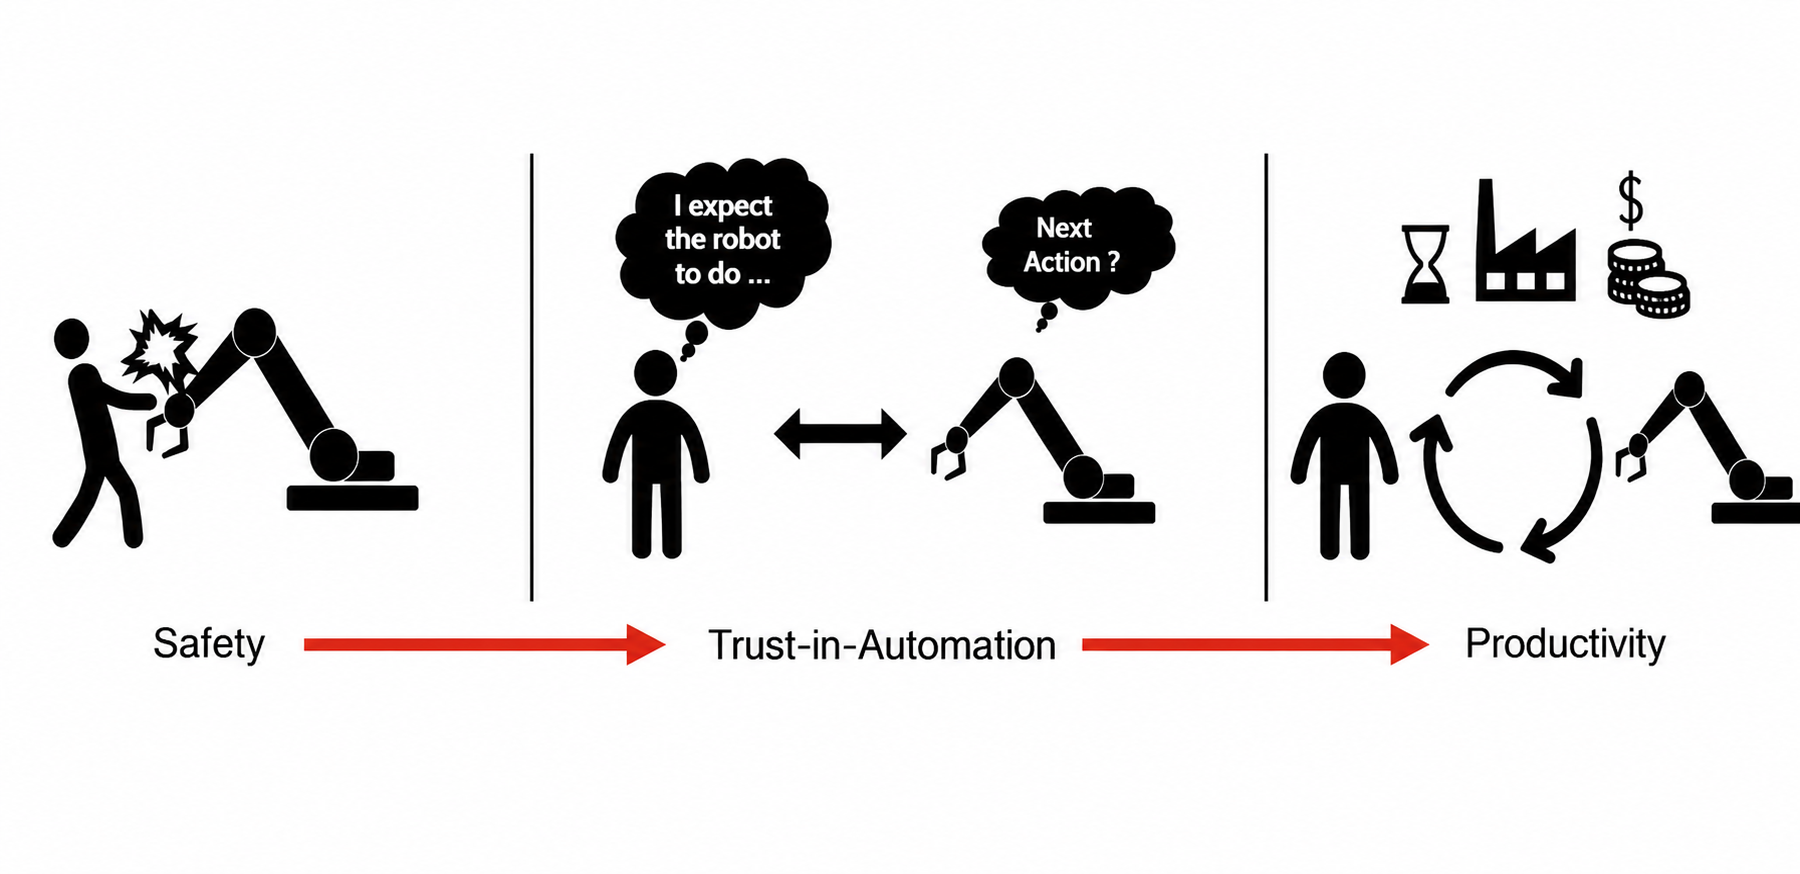
\includegraphics[width=\textwidth]{example_images/HRC_safety_productivity.png}
    \caption{Main challenges in HRC\cite{kumar2021hrc}.}
    \label{fig:hrc_challenges}
\end{figure}

}

\subsection{Conventional Risk Assessment and Risk Reduction}

{\small

Conventional risk assessment in robotic systems is generally performed before deployment and is based on the intended use, foreseeable misuse, system limits, operating environment, and known hazards of the system. According to ISO 12100, the risk assessment process includes hazard identification, risk estimation, and risk evaluation, followed by the selection of suitable risk reduction measures \cite{iso12100}. In the context of industrial and collaborative robots, this process is supported by robot-specific safety standards that define requirements for robot systems, collaborative applications, and protective measures \cite{iso10218_1_2025,iso10218_2_2025,iso15066}.

Risk reduction is usually implemented through a combination of inherently safe design, technical protective measures, and information for use. In HRC, this can include limiting robot speed and force, defining safe separation distances, using protective stops, and applying physical or electronic safeguards around the robot workspace. These measures are essential because they provide a systematic way to reduce the likelihood or severity of hazardous human-robot interactions before the system is put into operation.

However, conventional risk assessment is mainly based on assumptions made during design and deployment. These assumptions include expected human behaviour, known object configurations, defined workspaces, and predefined task conditions. As a result, conventional risk assessment is effective for identifying known and reasonably foreseeable hazards, but it becomes limited when the operating context changes significantly during runtime. This limitation is especially relevant for autonomous robotic systems, where the robot may operate in dynamic environments and make decisions based on sensor data and perception results.

}
\subsection{Existing Safety Measures in HRC}

{\small

In industrial HRC, risk reduction strategies are commonly implemented through two main approaches: the use of collaborative robots and the use of physical or electronic safeguarding measures \cite{kumar2021hrc}. Collaborative robots, also referred to as cobots, are designed to operate in direct cooperation with humans within a defined shared workspace. Their safety is supported through hardware and software features such as reduced momentum, force sensing, back-drivable actuators, and protective stop functions that interrupt robot motion when unexpected contact or resistance is detected.

The safeguarding-based approach focuses on monitoring the robot workspace so that robot motion can be adapted or stopped before hazardous human-robot collisions occur. In practice, this is achieved using physical and electronic safeguarding devices that define protected zones around the robot work cell. Examples include safeguarded perimeter door switches, light curtains, pressure-sensitive floors, 2-D scanning LiDAR, and 3-D safety vision systems. These mechanisms are important for reducing the risk of human injury, but they often rely on predefined safety zones, fixed distance thresholds, or conservative stopping rules \cite{kumar2021hrc}.

A common method used for workspace monitoring is Speed and Separation Monitoring (SSM). In SSM, the distance between the human and the robot is monitored continuously, and the robot speed is reduced or stopped when the separation distance becomes too small. In a static SSM approach, the monitored zones are usually predefined before operation. For example, a robot may operate at full speed when no human is detected in the outer zone, slow down when a human enters a warning zone, and stop when the human enters a protective stop zone\cite{kumar2021hrc}. This approach is simple and practical, but it can be conservative because the safety zones are not always adapted to the actual robot motion, human motion, task state, or sensor uncertainty.

\begin{figure}[htbp]
    \centering
    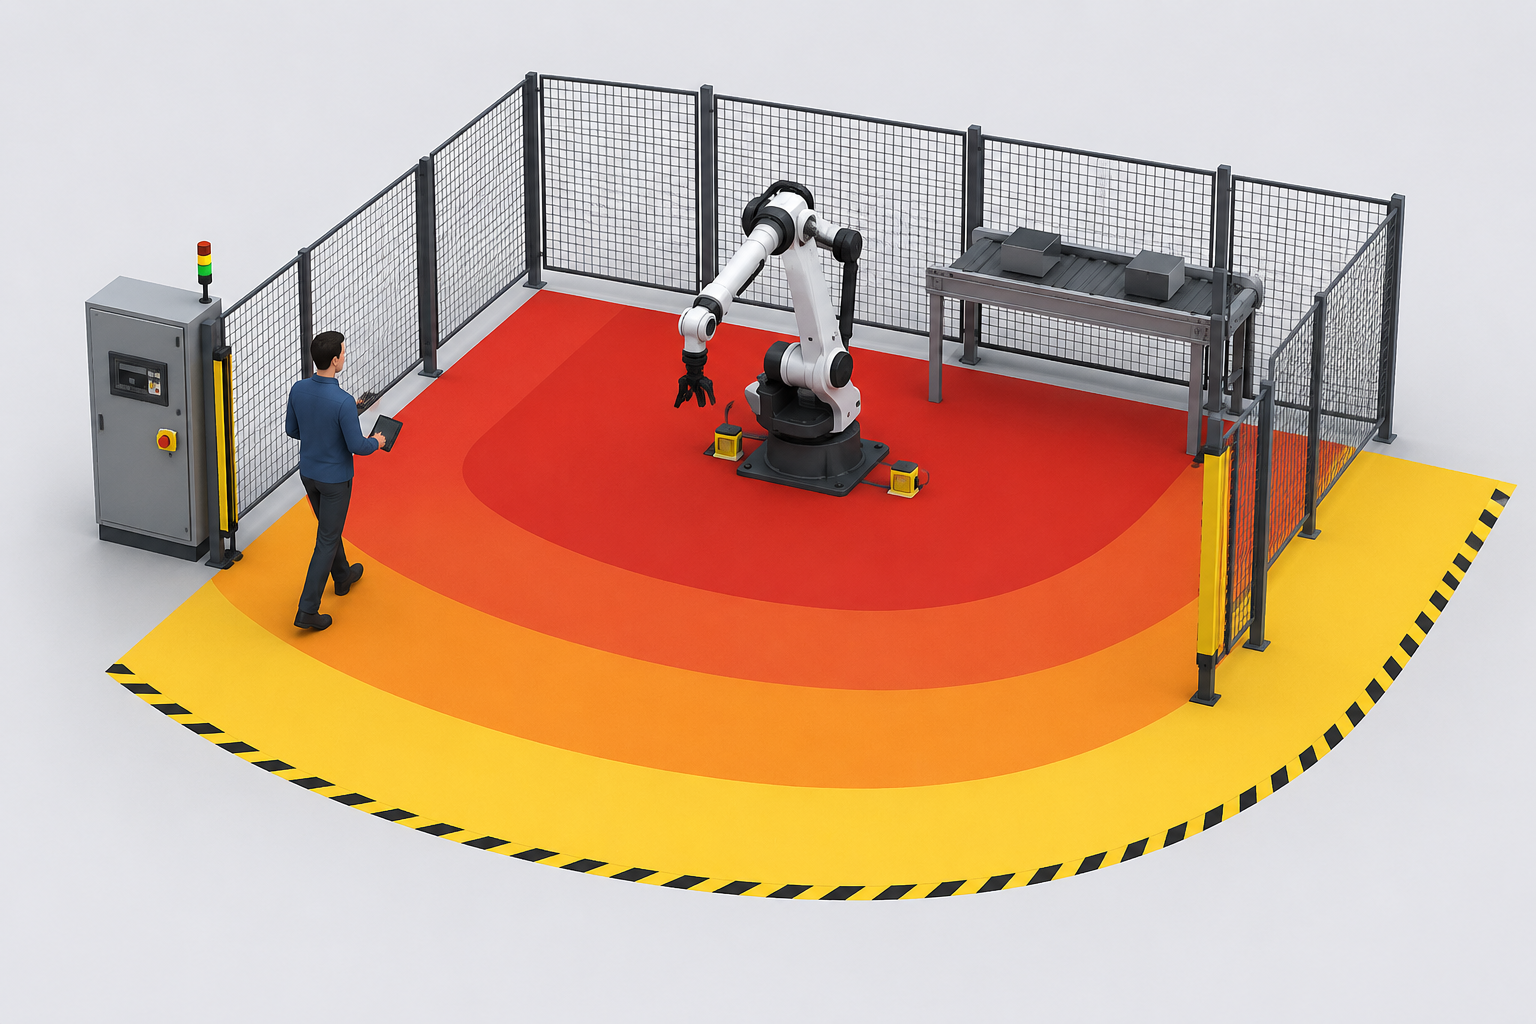
\includegraphics[width=\textwidth]{example_images/hrc_safety_zones_generated.png}
    \caption{Illustrative representation of safety zones in a collaborative robot workspace.}
    \label{fig:hrc_safety_zones}
\end{figure}

Dynamic SSM addresses this limitation by adapting the protective separation distance or the robot speed according to the current operating situation. Instead of relying only on fixed zones, dynamic SSM considers factors such as the actual distance between the human and the robot, robot velocity, human motion, stopping time, and uncertainty in the sensed position of obstacles or operators. Marvel discusses SSM performance in terms of both safety and productivity, representing collision potential through separation metrics and sensor uncertainty \cite{marvel2013ssm}. This shows that SSM is not only a binary stop-or-run mechanism, but also a method whose effectiveness depends on how accurately the system evaluates separation, uncertainty, and the productivity cost of safety actions.

Although dynamic SSM provides a more flexible basis for HRC safety than purely static safety zones, it also requires reliable perception, continuous monitoring, and suitable runtime decision-making. Therefore, existing safety measures show the importance of moving from fixed protective assumptions toward context-aware risk assessment mechanisms that can consider the actual operational situation of the robot, humans, and surrounding environment.

}

\subsection{Impact of Artificial Intelligence}

{\small

The previous subsections show that conventional risk assessment and many existing HRC safety measures are based on pre-deployment assumptions, such as intended use, expected human behaviour, known object configurations, predefined workspaces, fixed safety zones, and foreseeable hazardous scenarios. These assumptions are necessary for systematic risk assessment, but they become less reliable when autonomous robots operate in changing environments. Human positions, object locations, obstacles, task conditions, and spatial relationships may vary during operation, meaning that a risk analysis performed before deployment may no longer fully represent the actual operating situation.

The integration of artificial intelligence into robotic perception, planning, or control further increases this limitation. AI-based components can enable object detection, scene interpretation, motion prediction, task planning, and adaptive decision-making. While these capabilities improve flexibility and autonomy, they also make robot behaviour harder to predict completely during design-time safety analysis. Safety assurance of AI-based systems is complicated by dataset dependence, black-box behaviour, explainability, and lifecycle assurance \cite{silvaneto2022aisafetyassurance}. In robotic systems, this means that perception errors, low-confidence predictions, distribution shifts, previously unseen objects, changing human behaviour, or software updates after deployment can affect system decisions.

As a result, conventional risk assessment should be understood as a necessary baseline rather than a complete solution for adaptive autonomous robotic systems. If the deployed system operates under conditions that were not fully represented during the original assessment, the selected safety measures may become insufficient. Therefore, dynamic and context-aware risk assessment is required to incorporate runtime information such as robot state, human presence, object locations, spatial relationships, perception uncertainty, and environmental changes. Automated and continuous risk assessment has been proposed for software-defined robotic systems, where changes in software or system behaviour may require risk assessment to be updated during operation \cite{grimmeisen2023continuousrisk}.

At the same time, AI can also support dynamic risk assessment when its outputs are structured, bounded, and interpretable. AI-based perception and reasoning methods can help identify relevant objects, detect environmental changes, classify scene elements, and localise risk-relevant information around the robot. In this thesis, this motivates the use of a spatial risk-annotated scene graph, which can represent objects, spatial relations, uncertainty, and risk-related context in a machine-readable form to support dynamic risk assessment in autonomous robotic systems.

}














\section{Risk-Annotated Scene Graph Framework Baseline}

{\small

This section introduces the existing risk-annotated scene graph framework that forms the basis of this thesis \cite{previous_rsg_thesis}. The purpose is to explain the conceptual pipeline of the original work, including how visual input is processed, how objects and relationships are extracted, and how risk-related information is represented in the generated scene graph. This provides the necessary background for understanding the extensions proposed in this thesis.

The discussion focuses on the high-level concepts of the original framework rather than implementation-specific details. In particular, it describes the role of perception, segmentation, retrieval-augmented perception, vision-language model reasoning, scene graph construction, and risk annotation. The limitations of the existing framework are also considered, especially with respect to portability, scalability, spatial consistency, uncertainty representation, and runtime applicability.

}

\subsection{Information Flow in the Baseline Framework}


{\small

The baseline framework follows a modular processing pipeline in which RGB-D data is received, processed, interpreted, and integrated into a risk-annotated scene graph. The input to the system is an RGB-D observation of the environment, consisting of a colour image and its corresponding depth image. In the original implementation, this input can be provided through a dataset or submitted through an external interface. The external communication is handled through a FastAPI-based interface, which allows incoming samples and processing requests to be passed into the internal pipeline. This design separates data input and client communication from the perception and scene graph generation modules.

\begin{figure}[htbp]
    \centering
    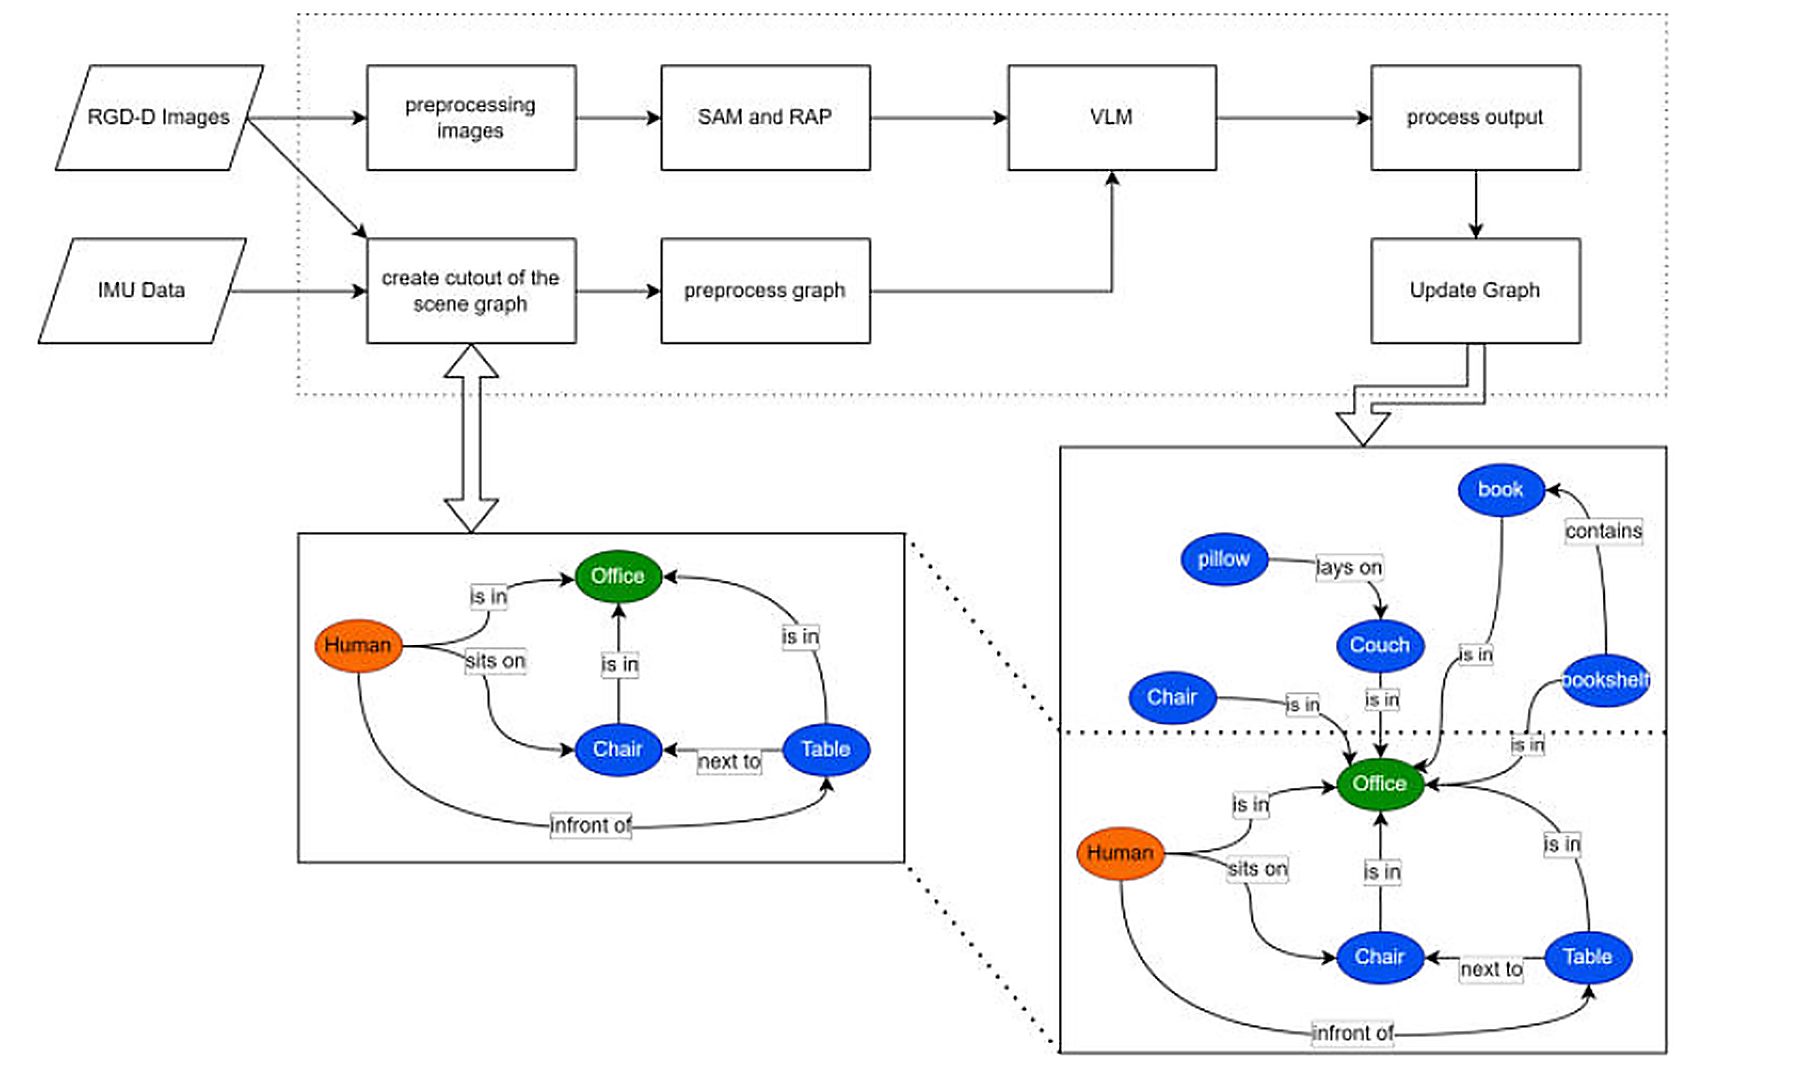
\includegraphics[width=\textwidth]{example_images/existing_work_overview_enhanced.png}
    \caption{Information flow of the existing risk-annotated scene graph framework. Adapted from \cite{previous_rsg_thesis}.}
    \label{fig:existing_rsg_framework}
\end{figure}

After an RGB-D input sample is received, the frame is handled as a task in the processing pipeline. The colour image is first used for object segmentation. For this purpose, the framework uses the Segment Anything Model (SAM) to generate object masks or image regions that may correspond to relevant entities in the scene. These masks are then used to create image cutouts for detected object candidates. The associated depth image, camera parameters, and pose information support later spatial processing, including coordinate conversion, visibility checking, and the spatial grounding of graph elements.

The segmented object candidates are then processed using a Retrieval-Augmented Perception (RAP) mechanism and a Vision-Language Model (VLM). RAP retrieves relevant or similar labels from a visual knowledge base for the detected object cutouts. This provides additional label candidates and prior visual context for the later interpretation stage. In parallel, the existing scene graph is reduced to a cutout that contains only the nodes and edges relevant to the current camera view. This scene-graph cutout is generated using the current pose and depth image, so that only likely visible graph elements are passed forward for inference.

The VLM receives the RGB image together with the scene-graph cutout and the possible labels retrieved for the detected object candidates. It is then used to interpret the current scene and produce structured information about visible entities, semantic labels, relationships, confidence values, and risk-relevant properties. The VLM output is parsed into a graph-like representation and then merged with the existing scene graph. During this update, existing nodes and edges can be modified, newly detected entities can be added, and graph information can be updated according to the latest observation.

Finally, the extracted and updated information is maintained as a risk-annotated scene graph. In this representation, relevant objects are modelled as nodes, while spatial, semantic, or risk-related relationships are represented as edges or attributes. The depth component of the RGB-D input is important because it supports spatial grounding of detected objects and enables approximate geometric relationships to be represented in the graph. The resulting graph provides a machine-readable representation of the observed scene and can be used as structured input for downstream reasoning or risk assessment. The overall information flow can therefore be summarised as RGB-D input, task handling, object segmentation, object cutout generation, RAP-based label retrieval, scene-graph cutout generation, VLM-based interpretation, and scene-graph update.

The main design elements of the baseline framework are its modular worker-based structure, its separation between external communication and internal processing, its use of foundation models for segmentation and semantic interpretation, its retrieval-based support for object labelling, and its graph-based representation of RGB-D scene information. These elements make the framework suitable as a basis for risk-aware scene understanding.

}
\subsection{FastAPI}

FastAPI is a modern Python web framework used for building application programming interfaces (APIs) \cite{fastapi_docs}. It allows external clients to communicate with a software system through network-accessible endpoints, typically using HTTP requests. In robotics and perception systems, this can be useful when a perception pipeline is executed as a separate service and must receive RGB-D observations, processing requests, or configuration information from external programs.

One advantage of FastAPI is that structured interfaces can be developed quickly in Python. The expected format of incoming requests can be defined explicitly, which is useful when external clients submit complex data such as RGB-D images, timestamps, and pose information. FastAPI also supports asynchronous web-server operation, making it suitable for service-based applications that handle multiple requests, communicate with external processes, or expose machine-learning components through a network interface \cite{fastapi_docs}. In the baseline risk-annotated scene graph framework, this provides a practical way to expose the scene graph generation pipeline as an external service while keeping the client application separated from the internal perception, segmentation, VLM, and scene graph modules.

However, a FastAPI-based interface also has limitations for direct integration with autonomous robotic systems. Robotic software usually requires continuous sensor streams, low-latency communication, synchronised multi-modal data, distributed robot nodes, and predictable timing behaviour. A REST-based API is well suited for request-response communication \cite{fastapi_docs}, but it is less natural for high-frequency RGB-D streams and real-time control loops. Therefore, FastAPI is useful as a modular service interface in the baseline framework, but it is not ideal as the primary communication mechanism for portable robotic deployment. This motivates the later porting of the framework to ROS 2, where RGB-D data, pose information, scene graph updates, and system status can be handled using robot-native communication mechanisms.


\subsection{SAM-Based Object Segmentation}

{\small

The Segment Anything Model (SAM) is a foundation model for image segmentation introduced by Kirillov et al. \cite{kirillov2023segmentanything}. It is designed as a promptable segmentation model that can generate masks from inputs such as points, bounding boxes, or masks. Since SAM is not limited to a fixed set of object classes, it is useful for open-ended visual perception tasks where the objects in a scene may not be known in advance.

In the baseline risk-annotated scene graph framework, SAM is used to extract candidate object regions from the RGB component of the RGB-D input. For each retained object candidate, the framework keeps an object crop, a bounding box, a binary segmentation mask, and a confidence-related score. The crop is used for later visual interpretation, the bounding box and mask describe the image-space extent of the object candidate, and the score indicates the quality or stability of the segmentation.

SAM therefore provides the low-level object proposal stage of the pipeline. However, it does not provide object identities, semantic relationships, risk labels, physical meaning, or 3D positions. Depth data, retrieval-based labels, and VLM-based interpretation are required before the segmented regions can be represented as meaningful nodes and relations in a risk-annotated scene graph.

}

\subsection{Retrieval-Augmented Perception}

{\small

Retrieval-Augmented Perception (RAP) in the baseline framework follows the broader idea of retrieval-augmented methods, where stored information is retrieved and used to support the interpretation of new input. This idea is closely related to retrieval-augmented generation, introduced by Lewis et al. for knowledge-intensive natural language processing tasks, where generated outputs are supported by information retrieved from an external knowledge source \cite{lewis2020rag}. In the baseline framework, this principle is transferred from text-based generation to visual perception. Instead of interpreting each segmented object only from the current RGB-D observation, the system retrieves relevant information from previously stored visual observations and uses it as additional context for object interpretation.

After SAM generates candidate object regions, these object cutouts are passed to the RAP mechanism. RAP compares the current visual object candidates with entries in a visual knowledge base and retrieves similar or relevant object labels. These retrieved labels act as prior information for the later VLM-based interpretation stage. In this way, RAP supports object consistency across observations and reduces the dependence on the VLM having to infer every object label from the current image alone.

The main advantage of RAP is that it introduces memory-like behaviour into the perception pipeline. If an object or a visually similar object has been observed before, the retrieved information can help guide the interpretation of the current scene. This is useful for risk-annotated scene graph generation because object identity and consistency are important when maintaining a structured representation of the environment over time. However, RAP does not independently solve object recognition or risk assessment. Its output must still be interpreted together with the current RGB-D observation, the segmented object regions, and the VLM output before the information can be inserted into the scene graph.

}

\subsection{Vision-Language Model Reasoning}


{\small

Vision-Language Models (VLMs) are multimodal models that combine visual and textual information to support image understanding through natural language. Unlike conventional object recognition models that predict labels from a fixed set of classes, VLMs can interpret visual content using prompts, descriptions, or structured instructions. Instruction-following VLMs such as LLaVA demonstrate how visual inputs can be connected with language-model reasoning through multimodal instruction tuning \cite{liu2023llava}. This makes VLMs useful for open-ended scene understanding, where the system must identify objects, infer relationships, and reason about context beyond predefined categories.

Within the baseline framework, the VLM acts as the semantic reasoning component. It converts visual and contextual information into structured scene-level outputs, including object identities, attributes, relationships, confidence values, and risk-relevant descriptions. These outputs provide the semantic information required for constructing and updating the risk-annotated scene graph.

The baseline study evaluated LLaVA 1.6 Mistral 7B, Qwen 2.5-VL 7B, and Phi-4 Vision Multimodal for the scene graph generation task. The comparison considered input- and output-format compatibility, repetition and hallucination behaviour, and the stability of location-format output. Based on this evaluation, the Qwen model series was identified as the best performing option for the baseline framework \cite{previous_rsg_thesis}. Later testing used Qwen 3-VL to use the newer available model version while preserving the framework's model-interchangeable design \cite{previous_rsg_thesis}.

However, VLM-based reasoning can produce inconsistent descriptions, miss small objects, or infer relationships that are not fully supported by the visual input. Therefore, VLM output cannot be treated as directly reliable safety information. It must be bounded, checked, and converted into a consistent graph representation before it can support downstream risk assessment. This motivates the refinement of VLM outputs in this thesis.

}

\subsection{Scene Graph Construction and Risk Annotation}

{\small
The baseline framework represents the scene graph as a directed graph, where entities in the environment are modelled as nodes and relationships between entities are modelled as edges \cite{previous_rsg_thesis}. The original implementation uses NetworkX, a Python library for network analysis and graph manipulation, which supports incremental graph operations such as adding, updating, and removing nodes and edges \cite{hagberg2008networkx}.

For external communication, the internal graph is converted into a dictionary-based representation. This is necessary because a native NetworkX graph object is not directly suitable for robust API transfer. The dictionary representation preserves the logical structure of the graph by storing node and edge information separately, making it easier to return through the FastAPI interface and process by external clients.

Each node stores semantic, spatial, and risk-related information. Important node attributes include a persistent identifier, object label, semantic description, semantic pose, 3D position, risk metadata, appearance score, confidence score, and layer type. The semantic description describes the visual identity of the entity, while the semantic pose describes its current physical state, such as standing, lying, open, closed, or moving. Edges store relationships between nodes, including the source node, target node, relationship label, and distance between the connected entities.

The graph update process must handle perception errors such as false positives and false negatives. To improve robustness, the baseline framework uses an appearance score-based graph combination strategy. When an object is repeatedly observed with consistent properties, its appearance score is increased. When it is missing from the latest VLM output, its score is decreased. A node is removed only when its appearance score falls below a predefined threshold, which prevents isolated missed detections from immediately deleting objects from the graph.

Overall, the scene graph construction strategy combines semantic information, spatial information, and risk-related metadata in a machine-readable representation. This makes the baseline framework suitable for incremental risk-aware scene understanding, while also motivating later extensions for spatial consistency, uncertainty handling, and scalability in larger environments.

}

\subsection{Limitations of the Baseline Framework}

{\small

Although the baseline framework provides a suitable foundation for risk-annotated scene graph generation, it has several limitations when considered for deployment in autonomous robotic systems. The first limitation is related to portability. The original framework is exposed mainly through a FastAPI-based service interface, which is useful for dataset-based testing and external client communication. However, autonomous robotic systems typically rely on robot middleware for continuous sensor streams, synchronised data exchange, distributed nodes, and runtime coordination. As a result, the baseline interface is not directly aligned with robot-native communication patterns, making integration with real robotic platforms less straightforward.

A second limitation concerns scalability across larger environments. The baseline framework processes RGB-D observations and updates a scene graph based on the current frame, camera pose, and visible graph elements. This is suitable for local scene understanding, but it does not by itself provide a complete mechanism for building and maintaining a spatially consistent graph across multiple rooms, corridors, or revisited locations. As the operating area increases, the system requires stronger spatial anchoring so that objects observed at different positions and times can be associated with the correct location in a global environment representation.

Closely related to this is the absence of a dedicated loop closure mechanism. In mobile robotic operation, the robot may revisit a previously observed area after accumulating pose drift. Without loop closure, the system may treat revisited objects or locations as new observations, or may update the scene graph using spatial information that is no longer globally consistent. This limits the framework's ability to maintain a reliable long-term scene graph in larger environments. For this reason, integration with SLAM-based spatial data and loop closure detection is necessary for extending the framework beyond local frame-by-frame scene understanding.

The baseline framework also has limitations with respect to uncertainty representation. Object candidates are generated from segmentation, interpreted by a VLM, and then merged into the scene graph using confidence-related and appearance-based information. This supports basic persistence handling, because objects that are repeatedly observed can be treated as more stable than objects that appear only briefly. However, this does not provide a full probabilistic representation of object existence, object class, or spatial position. For downstream risk assessment, such probabilistic information is important because the risk associated with an object may depend not only on its detected class, but also on the likelihood of its presence, the uncertainty of its location, and the reliability of its classification. Representing important objects with probability distributions or uncertainty estimates would allow the risk assessment mechanism to distinguish between confidently detected objects, weakly observed objects, and objects whose position or classification remains uncertain.

Finally, the baseline framework depends strongly on the quality and consistency of VLM output. VLM-generated scene graph information may contain formatting errors, hallucinated relationships, missed objects, or inconsistent descriptions. Although parsing and graph-combination mechanisms can reduce some of these effects, the output still needs to be bounded and checked before it can be used as reliable input for risk assessment. These limitations motivate the extensions proposed in this thesis: porting the framework to ROS 2, integrating SLAM-based spatial information and loop closure, introducing probabilistic object representation, refining VLM output constraints, and considering near-real-time operation during system design.

}




\section{Section3}
\small{


}
\section{Section4}
\small{


}
\section{Section5}
\small{


}
\section{Section6}
\small{


}
\section{Section7}
\small{


}